\chapter{Versuchergebnisse}
\label{chap:versuchergenisse}

% ----------------------------------------
% Sec: Vergleichsmessung von modifizierten Teilen
% ----------------------------------------
\section{Vergleichsmessung von modifizierten Teilen}
\label{sec:vergleichsmessung_von_difizierten_Teilen}

Zur Überprüfung der Funktion des neuen Systems, werden die Schmierfilmhöhen gegenübergestellt, die einerseits mit den modifizierten und anderseits mit den originalen Teilen (Kugel + Support) gemessen werden.
Außerdem werden diese Messergebnisse mit den von theoretischer Berechnung verglichen.

Die Vergleichsmessung wird mit dem Mineralöl \textit{FVA 3} bei der Temperatur von \SI{40}{\degreeCelsius} und der Last von \SI{20}{\N} durchgeführt (siehe Abbildung~\ref{fig:vergleichsmessung}).
Man kann hier sehen, dass das neue System gut funktioniert.

% ----------------------------------------
% Fig: Vergleichsmessung von neuer Kugel + neuer Scheibe,
% neuer Kugel + alte Scheibe und theoretische Filmdicke
% ----------------------------------------
\begin{figure}[htb]
    \centering
    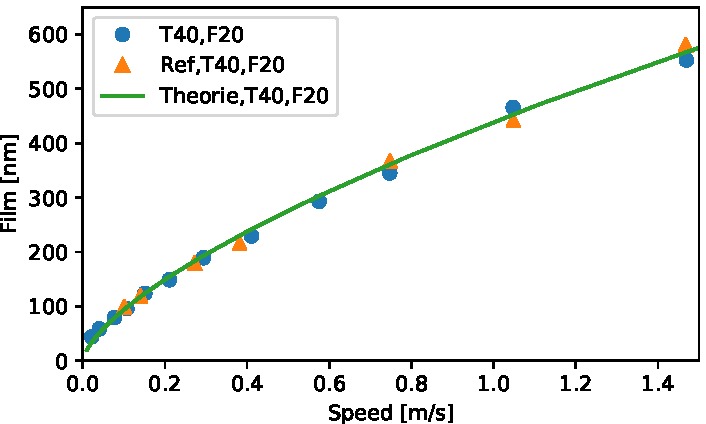
\includegraphics[]{./images/vergleichsmessung_T40_F20_FVA3.pdf}
    \caption{Filmdicke von zwei Konfigurationen --- neue Kugel + neue Scheibe (rund); originale Teile (dreieckig); rechnerische Filmdicken (gerade) --- mit dem Öl \textit{FVA 3} bei $T =$ \SI{40}{\degreeCelsius} und $F =$ \SI{20}{\N}}
    \label{fig:vergleichsmessung}
\end{figure}

% ----------------------------------------
% Sec: Störkapazitätmessung
% ----------------------------------------
\section{Störkapazitätsmessung}
\label{sec:stoerkapazitaetsmessung}

Da die kapazitiven Messungen von elektrischen Störungen, die von Elektrogeräten im Labor enstehen, sehr empfindlich sind, werden die Kabel so kurz wie möglich gehalten.
Alle elektronischen Anschlüsse und Bauteile werden nah zu einander auf einer Platine gebaut.
Trotz dieser Maßnahmen kann man leider nie die Störungen eliminieren.
Aus diesem Grund wird diese ungewünschte Größen bzw. Störkapazität bei stationären Zustand, mit alle benötigen Geräten angemacht werden, gemessen.
Diese beträt ca. \SI{89}{\pico\farad} und wird danach von den Messergebnissen abgezogen.
Abbildung~\ref{fig:vergleichsmessung} zeigt die Bestimmung der Störkapazität an.

% ----------------------------------------
% Fig: Background capacitance
% ----------------------------------------
\begin{figure}[htb]
    \centering
    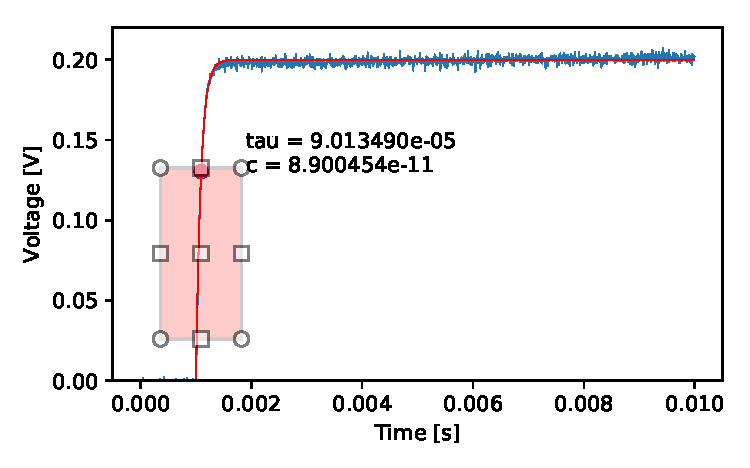
\includegraphics[]{./images/background_capacitance.pdf}
    \caption{Bestimmung der Störkapazität bevor einem Versuch: Messdaten (blau); angepasste Kurve (rot)}
    \label{fig:background_capacitance}
\end{figure}

% ----------------------------------------
% Sec: Kapazitätsmessung für EHD-Punktkontakt
% ----------------------------------------
\section{Kapazitätsmessung für EHD-Punktkontakt}
\label{sec:kapazitaetsmessung_punktkontakt}

% ----------------------------------------
% Fig: Kapazitätsmessung bei verschiedenen Temperaturen
% ----------------------------------------
\begin{figure}[htb]
    \centering
    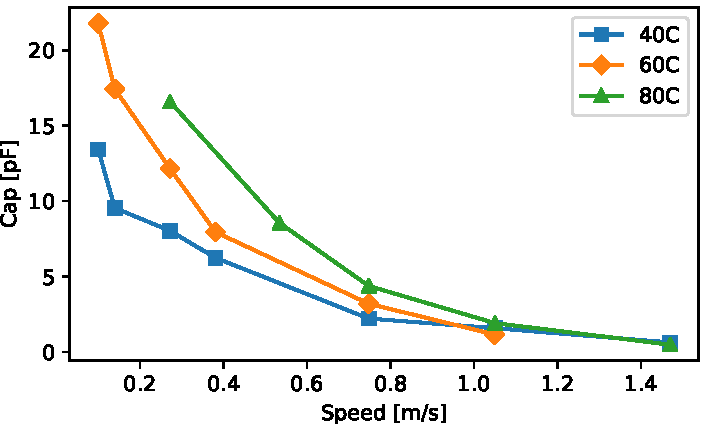
\includegraphics[]{./images/cap_vs_speed_dif_temp_meas.pdf}
    \caption{Kapazitätsmessung für das Mineralöl \textit{FVA 3} bei unterschiedlichen Temperaturen und einer Last von \SI{20}{\N}}
    \label{fig:cap_vs_speed_dif_temp_meas}
\end{figure}

% ----------------------------------------
% Fig: Kapazitätsmessung bei 40C
% ----------------------------------------
\begin{figure}[htb]
    \centering
    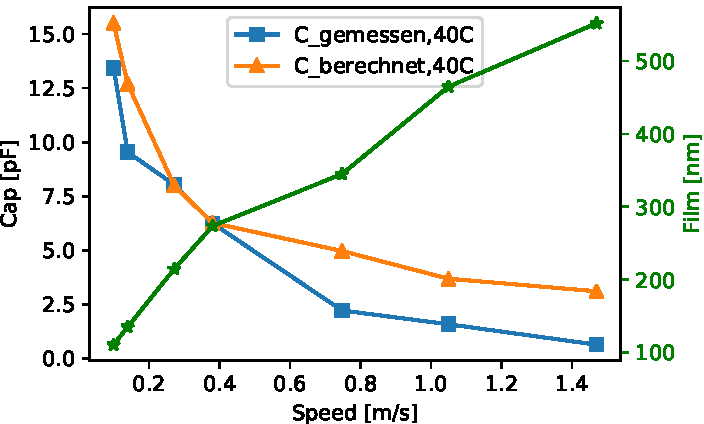
\includegraphics[]{./images/cap_theo_meas_vs_speed_40C.pdf}
    \caption{gemessenen Kapazitäten im Vergleich mit rechnerischen bei aufgenommen Filmhöhen von dem Öl \textit{FVA 3} bei $T =$ \SI{40}{\degreeCelsius} und $F =$ \SI{20}{\N}}
    \label{fig:cap_meas_cap_theo_40C}
\end{figure}

% ----------------------------------------
% Fig: Kapazitätsmessung bei 60C
% ----------------------------------------
\begin{figure}[htb]
    \centering
    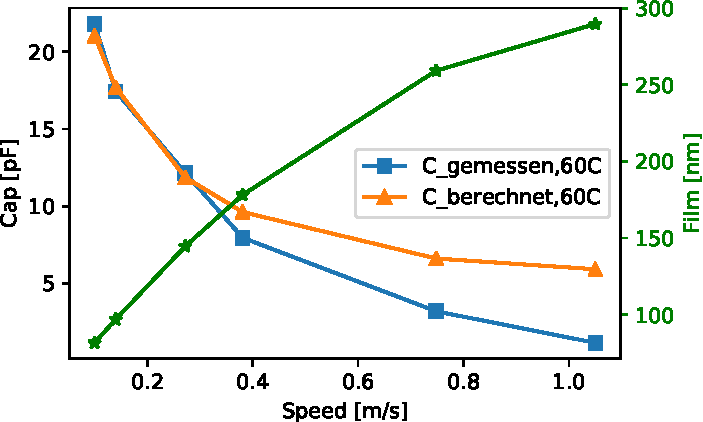
\includegraphics[]{./images/cap_theo_meas_vs_speed_60C.pdf}
    \caption{gemessenen Kapazitäten im Vergleich mit rechnerischen bei aufgenommen Filmhöhen von dem Öl \textit{FVA 3} bei $T =$ \SI{60}{\degreeCelsius} und $F =$ \SI{20}{\N}}
    \label{fig:cap_meas_cap_theo_60C}
\end{figure}

% ----------------------------------------
% Fig: Kapazitätsmessung bei 80C
% ----------------------------------------
\begin{figure}[htb]
    \centering
    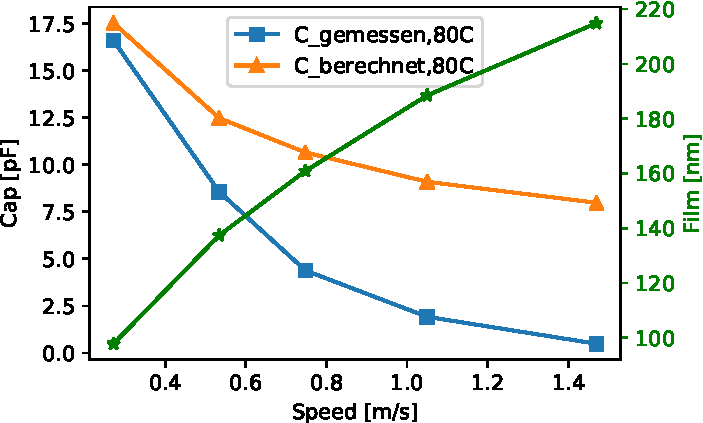
\includegraphics[]{./images/cap_theo_meas_vs_speed_80C.pdf}
    \caption{gemessenen Kapazitäten im Vergleich mit rechnerischen bei aufgenommen Filmhöhen von dem Öl \textit{FVA 3} bei $T =$ \SI{80}{\degreeCelsius} und $F =$ \SI{20}{\N}}
    \label{fig:cap_meas_cap_theo_80C}
\end{figure}
